\chapter{Conclusions and recommendations}

\label{chap-seven}

The research described in this dissertation aimed to develop the Condition Dependent Performance-Based Design methodology. First, an experimental program was conducted in which the stress-strain behavior and maximum bending strain of corroded reinforcing steel were obtained. The analytical program was then developed based on the outcomes of this experimental program. Second, in the analytical program, an SDOF cantilever column was developed using the open-source structural software OpenSeesPy \cite{Zhu2018}, in which the influence of corrosion level on the performance of the column was investigated. Finally, the results obtained from the experimental program and the analytical program were combined in a design and assessment example. The following sections summarize each phase of this research and highlight key observations. The final section outlines recommendations for future research related to this topic.

\section{Conclusions}
\subsection{Experimental Program}
\begin{itemize}
    \item The results obtained from tension tests performed on corroded reinforcing steel showed the effect corrosion has on the effective mechanical properties of the corroded reinforcing steel. The specimens were prepared by first developing the passive layer and later corroded to the specified corrosion level.
    \item The effective mechanical properties of the corroded reinforcing steel can are expressed here:
    \begin{equation}
        f_{y,CL} = f_{y,o}(1-0.0075CL)
        \label{eq.Calderon_Fy_vs_CL_ch7}
    \end{equation}
    
    \begin{equation}
        f_{u,CL} = f_{u,o}(1-0.0075CL)
        \label{eq.Calderon_Fu_vs_CL_ch7}
    \end{equation}

    \item The buckled bar tension tests developed in this research showed that as the corrosion level increases, the maximum bending strain decreases substantially, as can be observed in \fref{fig:BBT_strains_ch7}.
    
    \begin{figure}[htbp]
	    \centering
	    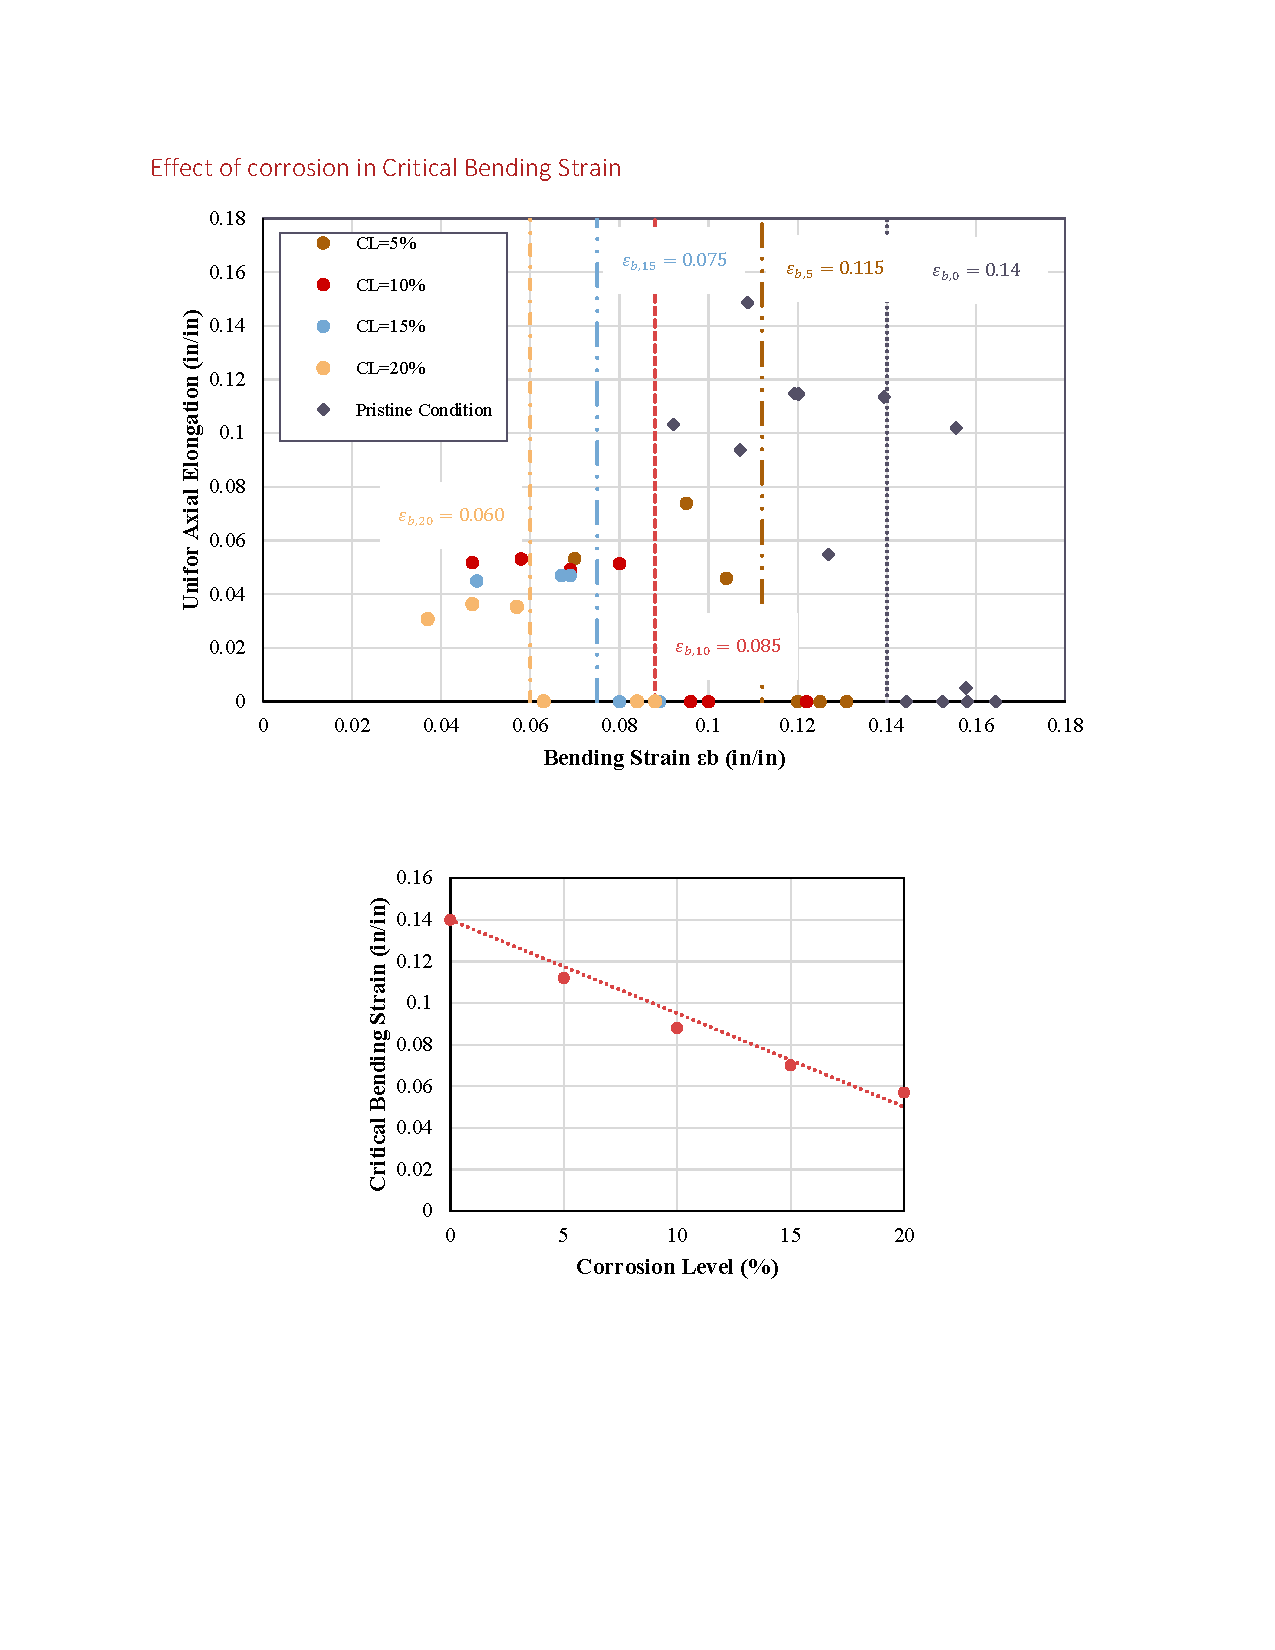
\includegraphics[width=0.95\textwidth]{VAC Thesis 2.0/Chapter-4/figs/BBT_results_.pdf}
	    \caption{Bending strain at different corrosion levels}
	    \label{fig:BBT_strains_ch7}
    \end{figure}
    
    The expression that relates corrosion level and maximum bending strain is shown here:
    \begin{equation}
        \varepsilon_{b}(CL) = \varepsilon_{o}-0.0045CL
        \label{eq.Calderon_eb_vs_CL_ch7}
    \end{equation}
    
    \item The SEM observations showed that chloride attach did not onset the fracture of rebars. As the tests on bars with removed imperfections confirmed, the geometrical imperfections caused by corrosion affect the observed behavior on the corroded reinforcing steel. The results from the tension tests on uncorroded reinforcing steel are shown below
\end{itemize}
\subsection{Analytical Program}
\begin{itemize}
    \item The analytical program showed that at a corrosion level of 10\% or higher there is an increase in the likelihood that a structure will achieve a limit state, as shown in \fref{fig:mean_prob_vs_CL_ch7}.
    
    \begin{figure}[htbp]
	\centering
	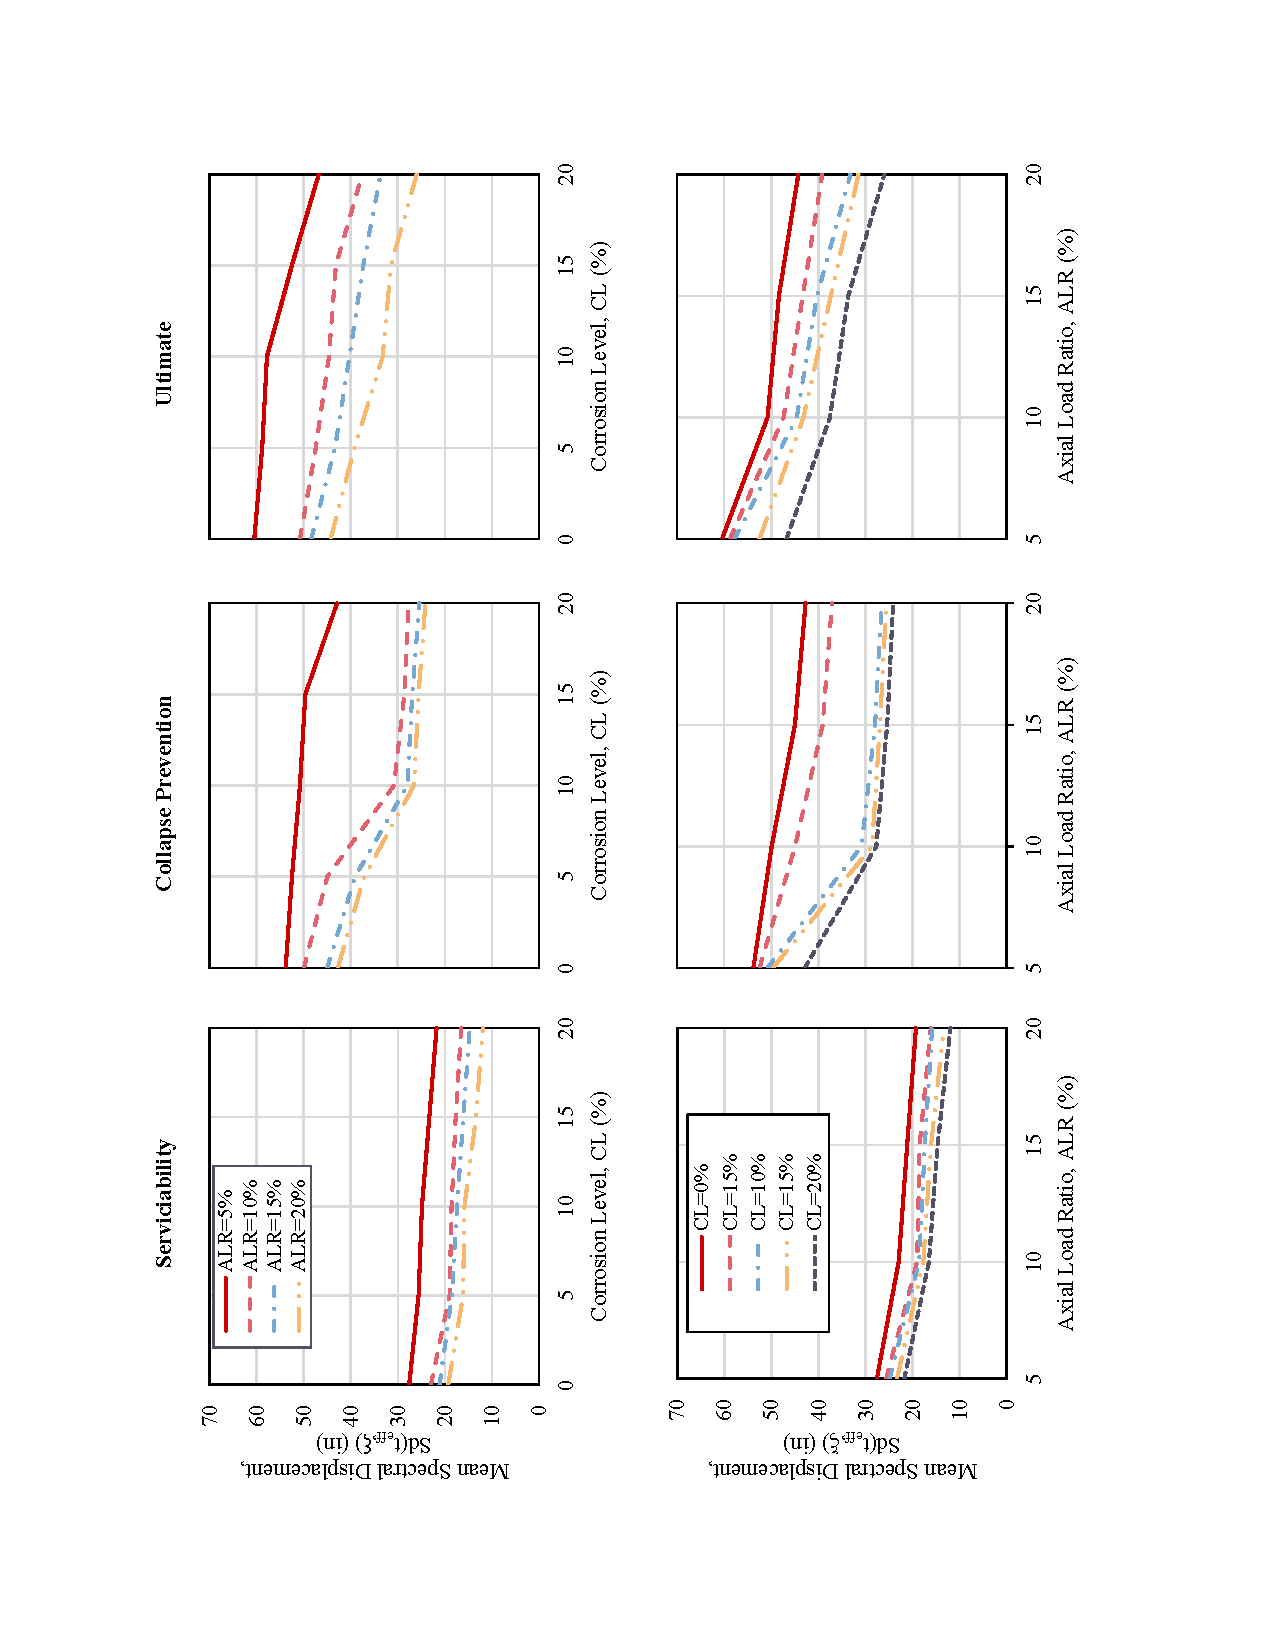
\includegraphics[width=0.85\textwidth]{VAC Thesis 2.0/Chapter-5/figs/Analysis_of_Mean_SDs.pdf}
	\caption{Analysis of mean values $(P=0.5)$ for performance limit states}
	\label{fig:mean_prob_vs_CL_ch7}
    \end{figure}
    
    \item As a result of this analysis, recommendations for the design and assessment of a structure are made: For the design of new structures, the corrosion level of a structure during the life service should not exceed 10\%. Similarly, for the assessment of existing structures, the DDBA methodology explained in this research can be used for corrosion levels of 10\% or lower. If an existing structure has a value of corrosion level greater than 10\%, a more refined procedure such as NLTHA is recommended.
\end{itemize}

\subsection{Condition Dependent Performance-Based Design and Assessment}
\begin{itemize}
    \item Although there are tools that allow the design of new structures to reduce the likelihood of corrosion occurring. The approach proposed in this research shows a simple method in which corrosion can be included to check that the structure will remain safe even as it corrodes.
    \item Similarly, the application of the findings from the experimental program showed that including the effect of corrosion in the assessment of bridges is feasible by including the effective mechanical properties of the reinforcing steel.
\end{itemize}

\section{Recommendations}

While this research shows that it is possible to design and assess structures to the effect of aging conditions, it is also clear that there is a need to understand the effect of aging on existing structures.

In addition, this research performed tests at the material level only. Therefore large-scale tests on corroded RC columns are necessary to verify the limit state expressions used for the design and assessment of structures. 

Another possible avenue of research is to perform large-scale tests that simulate aging conditions with materials related to different eras, i.e., structures with detailing and materials for the 1910-1950, 1950-1970, 1980-present. 

Finally, it is essential to understand at the regional level the effect these structures from different eras of design will have on the resiliency of cities across the United States as structures continue to age and new hazards such as climate change increase the threat of structural deterioration in combination with seismic, wind, and other types of loading.